\section{Betriebsführung}
    \begin{center}
        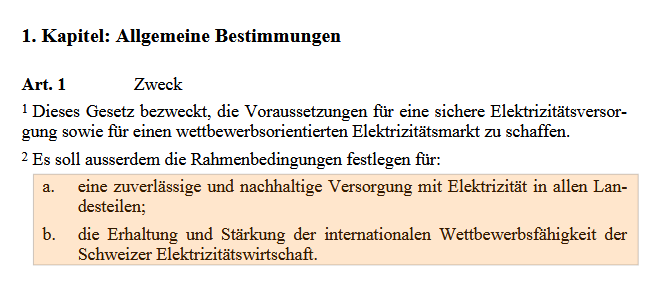
\includegraphics[width=0.9\columnwidth]{images/StromVG.png}
    \end{center}

    \begin{minipage}[t]{0.65\columnwidth}
        \centering \vspace{-0.7\baselineskip}
        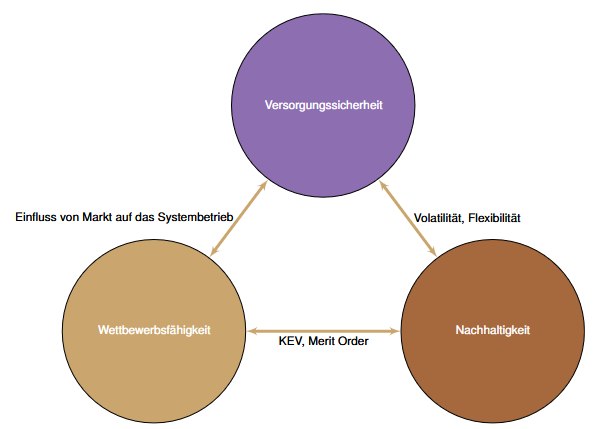
\includegraphics[width=0.85\linewidth]{images/Versorgung_Wettbewerb_Nachhaltig.png}
    \end{minipage}%
    \hfill
    \begin{minipage}[t]{0.34\columnwidth}
        \textbf{Versorgungssicherheit:}
        \begin{itemize}
            \item Räumlicher Ausgleich
            \begin{itemize}
                \item Netzbetriebsplanung
                \item Netzführung
                \item Engpassmanagement
                \item Transportkapazitäten
                \item Netzausbau
            \end{itemize}
            \item Zeitlicher Ausgleich
            \begin{itemize}
                \item Fahrplanmanag.
                \item Netzregelung
                \item Systemstabilität
                \item \dots
            \end{itemize}
        \end{itemize}
    \end{minipage}

    \begin{minipage}[t]{0.49\columnwidth}
        \textbf{Wettbewerbsfähigkeit:}
        \begin{itemize}
            \item Strommarkt
            \item Netznutzung
            \item Bilanzgruppensystem
            \item Kapazitätsallokationen
            \item \dots
        \end{itemize}
    \end{minipage}%
    \hfill
    \begin{minipage}[t]{0.49\columnwidth}
        \textbf{Nachhaltigkeit:}
        \begin{itemize}
            \item Kernausstieg
            \item volatile Erneuerbare Energieerzeugung (EE)
            \item Kostendeckende Einspeisevergütung
            \item \dots
        \end{itemize}
    \end{minipage}

\subsubsection{Besonderheiten von Strom}
    \begin{center}
        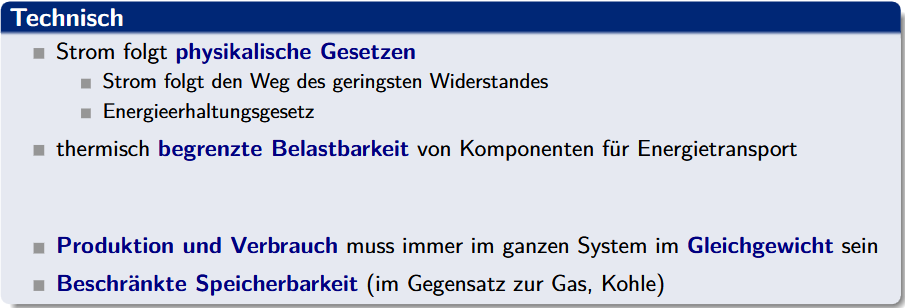
\includegraphics[width=.9\columnwidth]{images/Besonderheiten-technisch.png}
    \end{center}

    \begin{center}
        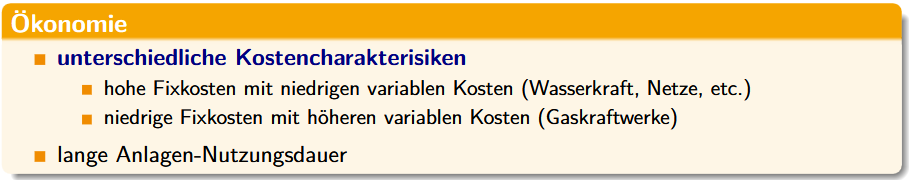
\includegraphics[width=.9\columnwidth]{images/Besonderheiten-ökonomisch.png}
    \end{center}

\subsection{Technische Sicht}
    \begin{center}
        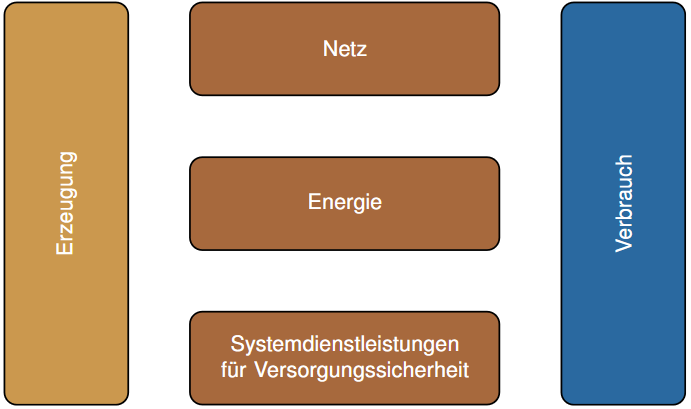
\includegraphics[width=.6\columnwidth]{images/Technisch-Übersicht.png}
    \end{center}

    \subsubsection{Technische Ziele (zu jedem Zeitpunkt)}
        \begin{itemize}
            \item Systemdienstleistungen
            \begin{itemize}
                \item Leistungsbilanz: \textit{Angebot = Nachfrage}
                \item Synchronizität: \textit{gleiche Frequenz an allen Knoten}
                \item Frequenzstabilität: \textit{Frequenz = 50 Hz}
                \item Spannungsstabilität: \textit{Spannung = Nennspannung}
            \end{itemize}
            \item Netzinfrastruktur
            \item Engpassmanagement
        \end{itemize}

    \subsubsection{Technische Herausforderungen}
        \begin{itemize}
            \item Variabilität: \textit{Fluktuierende Last- und Angebotsverläufe}
            \item Unsicherheit: \textit{Ungenaue Last- und Angebotsvorhersagen}
            \item Störungen: \textit{Ausfälle, Leistungsoszillationen, Blackouts}
        \end{itemize}

    \subsubsection{Systembetrieb: Arbeitsfelder}
        \begin{itemize}
            \item Grundenergiebeschaffung
            \begin{itemize}
                \item Marktbasierte Beschaffung
                \item Verschiedene räumliche Ebenen (Regional, nationale und international)
                \item Verschiedene Zeitebenen (Langfristige Verträge, Terminmarkt, Day-ahead, Intra-day)
            \end{itemize}
            \item Systemdienstleistungen
            \begin{itemize}
                \item Umfasst alle Produkte und Massnahmen die nicht zur Grundenergiebeschaffung gehören
                \item Kann marktbasiert oder regulatorisch umgesetzt werden
                \item Verschiedene räumliche und zeitliche Ebenen
                \item Regelenergie (Primär, Sekundär, Tertiär)
                \item Schwarzstartfähigkeit, Messungen, Blindleistung, Dämpfung und Schwungmasse
            \end{itemize}
        \end{itemize}

    \subsubsection{Systembetrieb: Aufgaben}
        \begin{itemize}
            \item Sicherstellung der technischen Ziele
            \item Wirtschaftlicher, kosteneffizienter Systembetrieb
            \item Faire Regeln für alle Netzakteure 
            \item[] (Erzeuger, Verbraucher, Netzbetreiber, Aggregatoren, ...)
            \item Berücksichtigung nationaler und internationaler politischer Interessen
            \item Unabhängige Prüfung der Sicherheitsaspekte
            \item Langfristige Planung und Weiterentwicklung des Systembetriebs
        \end{itemize}

\subsection{Marktsicht}
    \subsubsection{Ökonomische Analyse}
        \begin{itemize}
            \item verschiedene ökonomische Eigenschaften
            \item unterschiedliche Eignung für den Wettbewerb
            \item Elektrizitätsnetze hoher Investitionsbedarf 
            \item[] $\Rightarrow$ finanzielles Risiko $\Rightarrow$ Barriere für Investoren
            \item Produktion und Handel für Wettbewerb geeignet
            \begin{itemize}
                \item Erbringung ihrer Dienstleistungen abhängig vom Elektrizitätsnetzen
                \item Gewährleistung diskriminierungsfreien Zuganges zum Elektrizitätsnetzwerk
            \end{itemize}
        \end{itemize}

        \begin{center}
            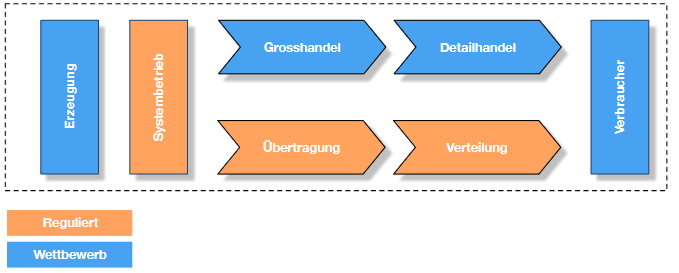
\includegraphics[width=0.8\columnwidth]{images/ökonomische-analyse.png}
        \end{center}

    \begin{minipage}[t]{0.49\columnwidth}
        \subsubsection{Monopol}
        \centering \vspace{-0.7\baselineskip}
        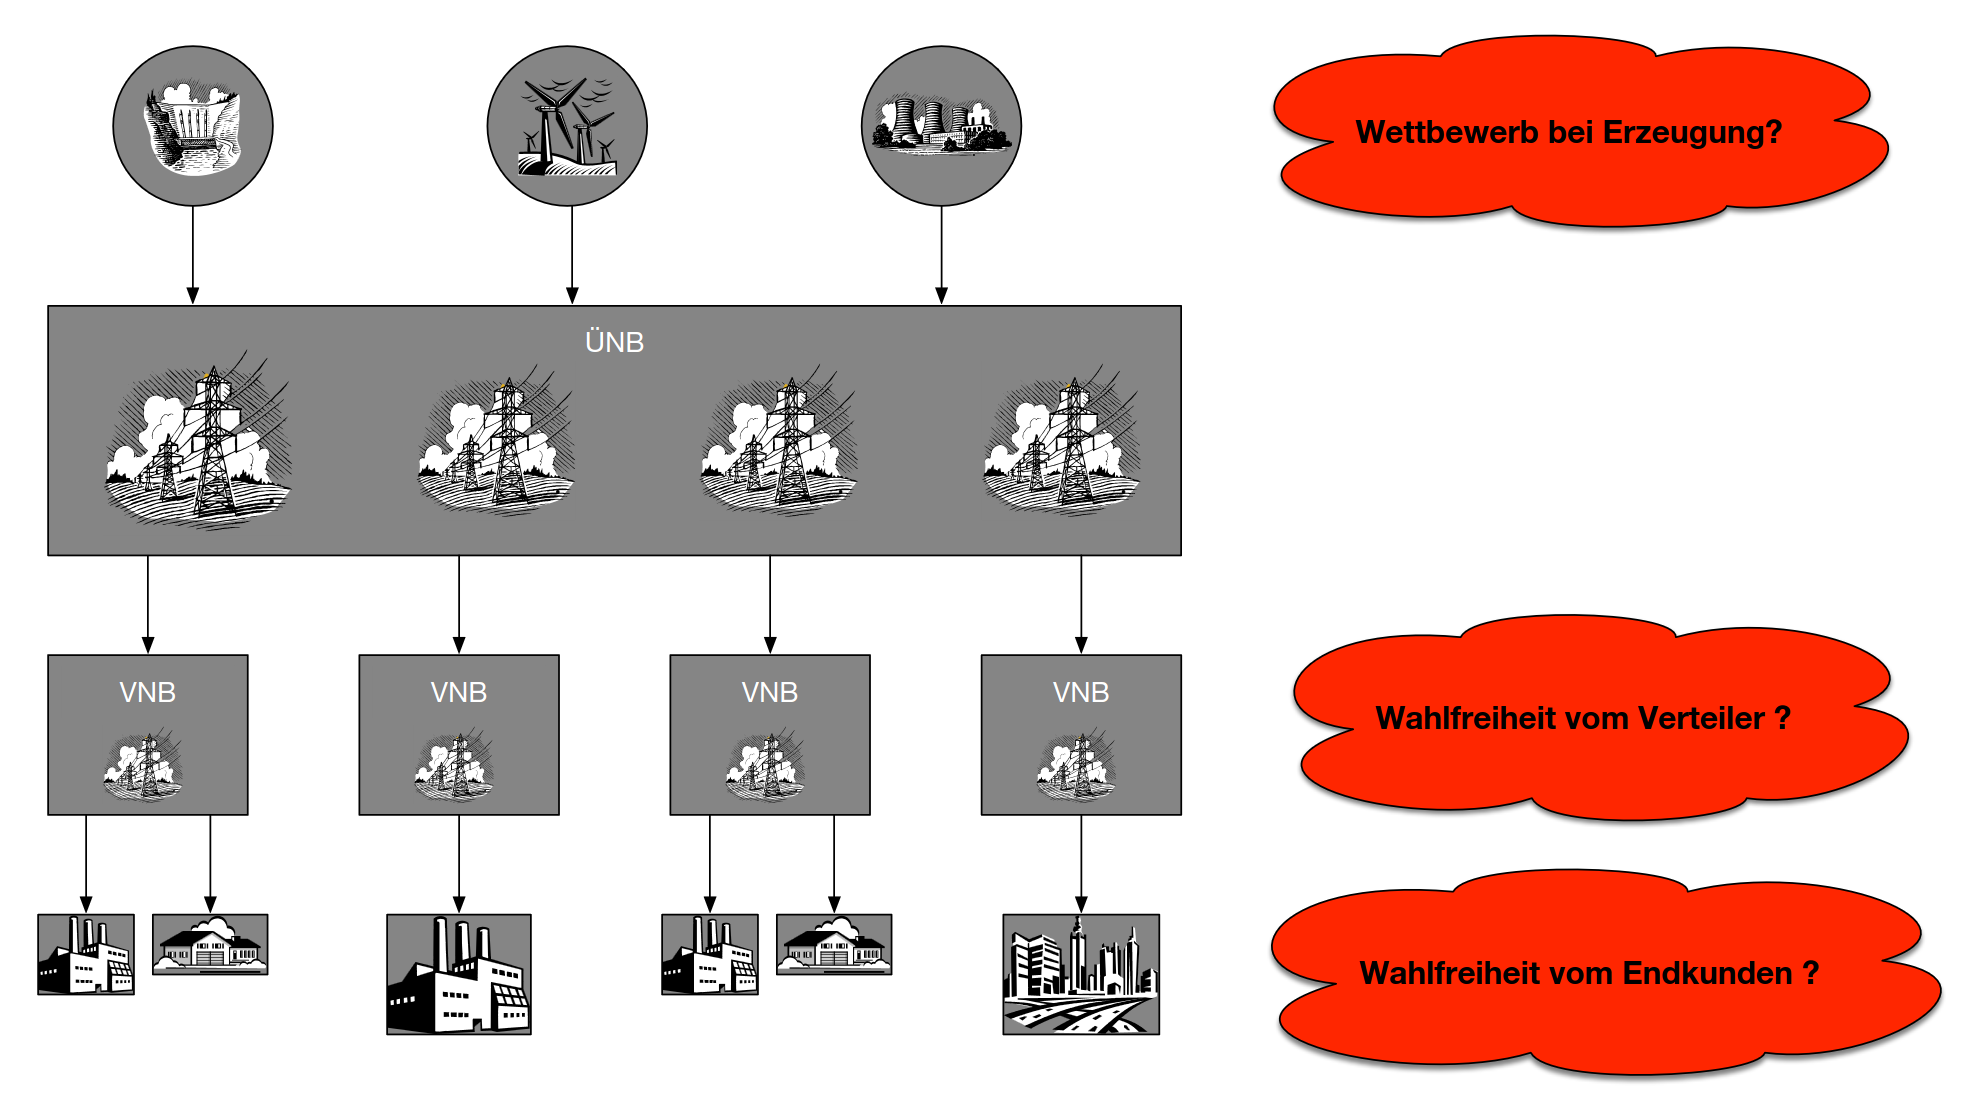
\includegraphics[width=0.95\linewidth]{images/Monopol.png}
    \end{minipage}%
    \hfill
    \begin{minipage}[t]{0.49\columnwidth}
        \subsubsection{Alleinabnehmer}
        \centering \vspace{-0.7\baselineskip}
        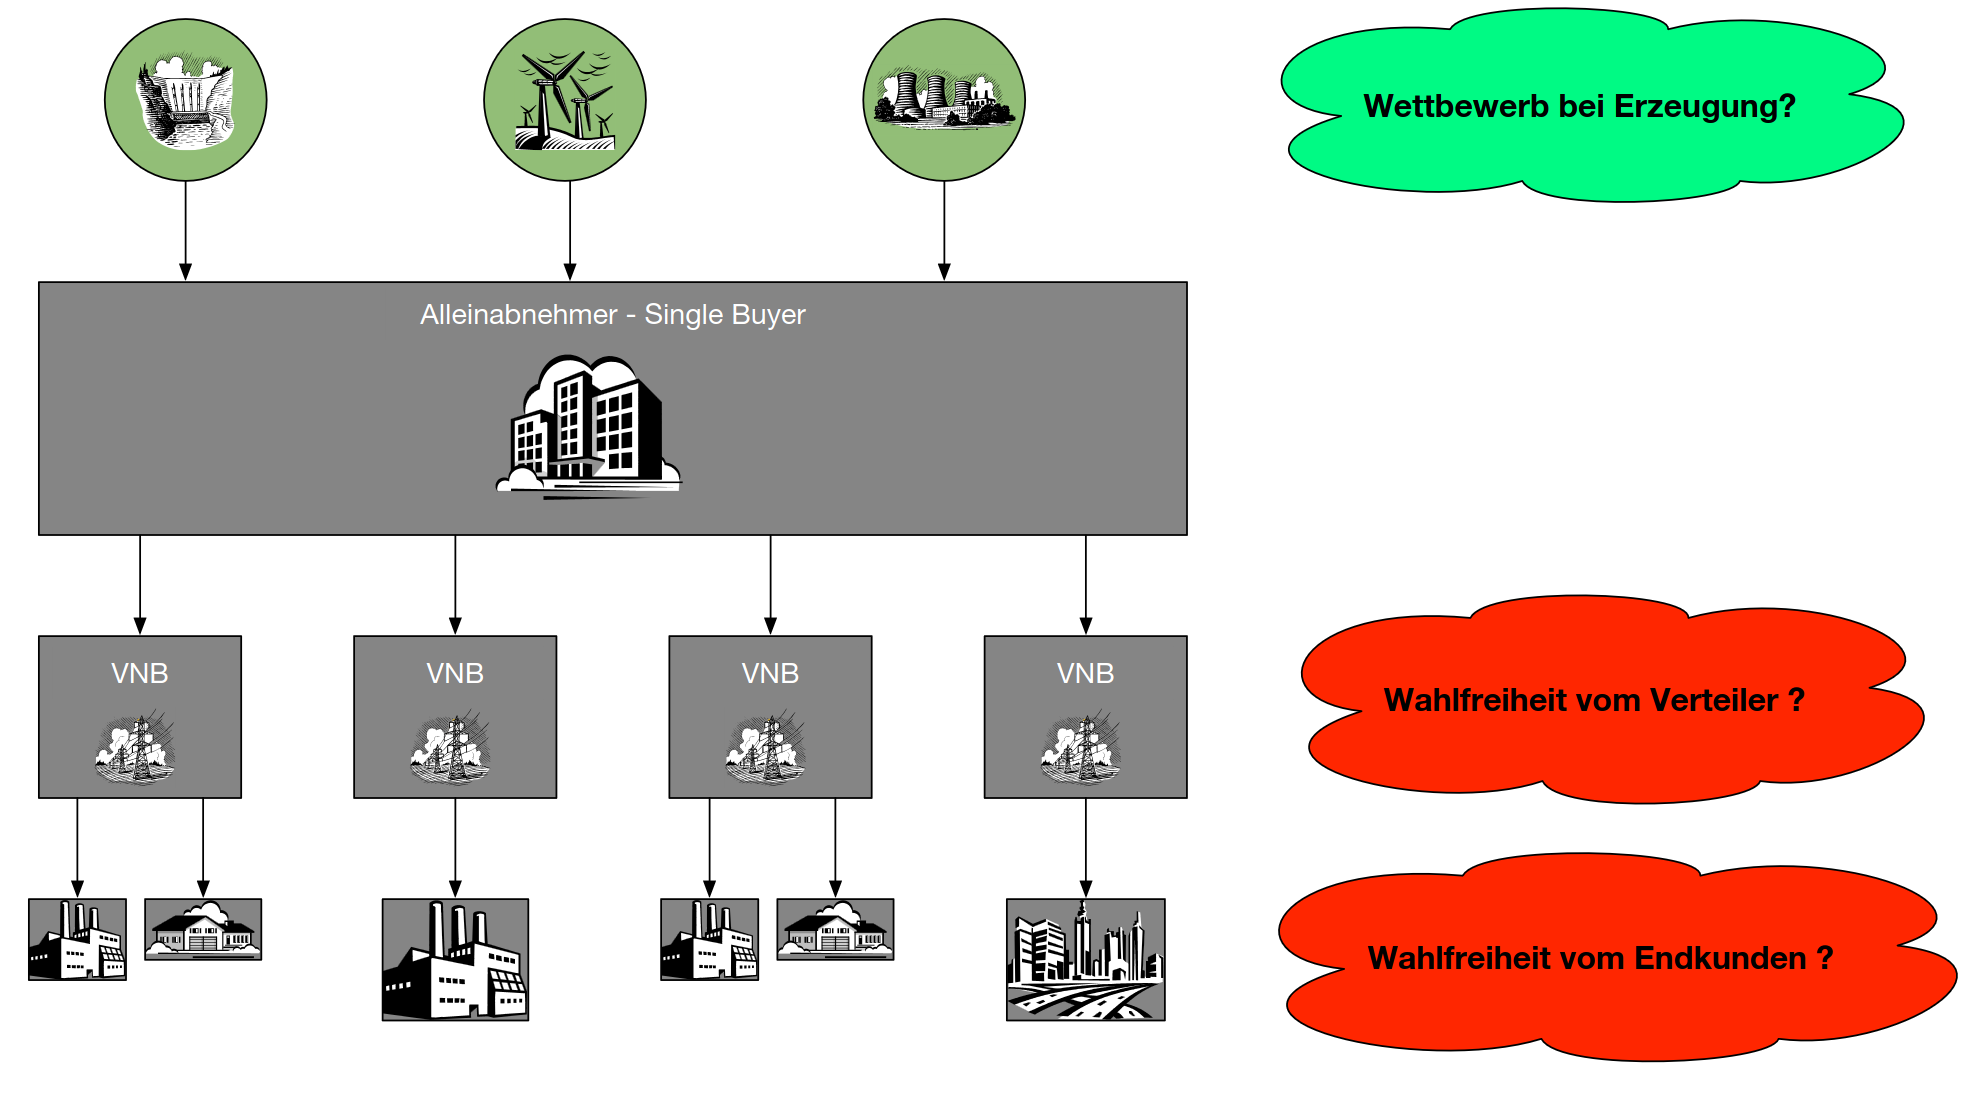
\includegraphics[width=0.95\linewidth]{images/alleinabnehmer.png}
    \end{minipage}

    \begin{minipage}[t]{0.49\columnwidth}
        \subsubsection{Grosshandelmarkt}
        \centering \vspace{-0.7\baselineskip}
        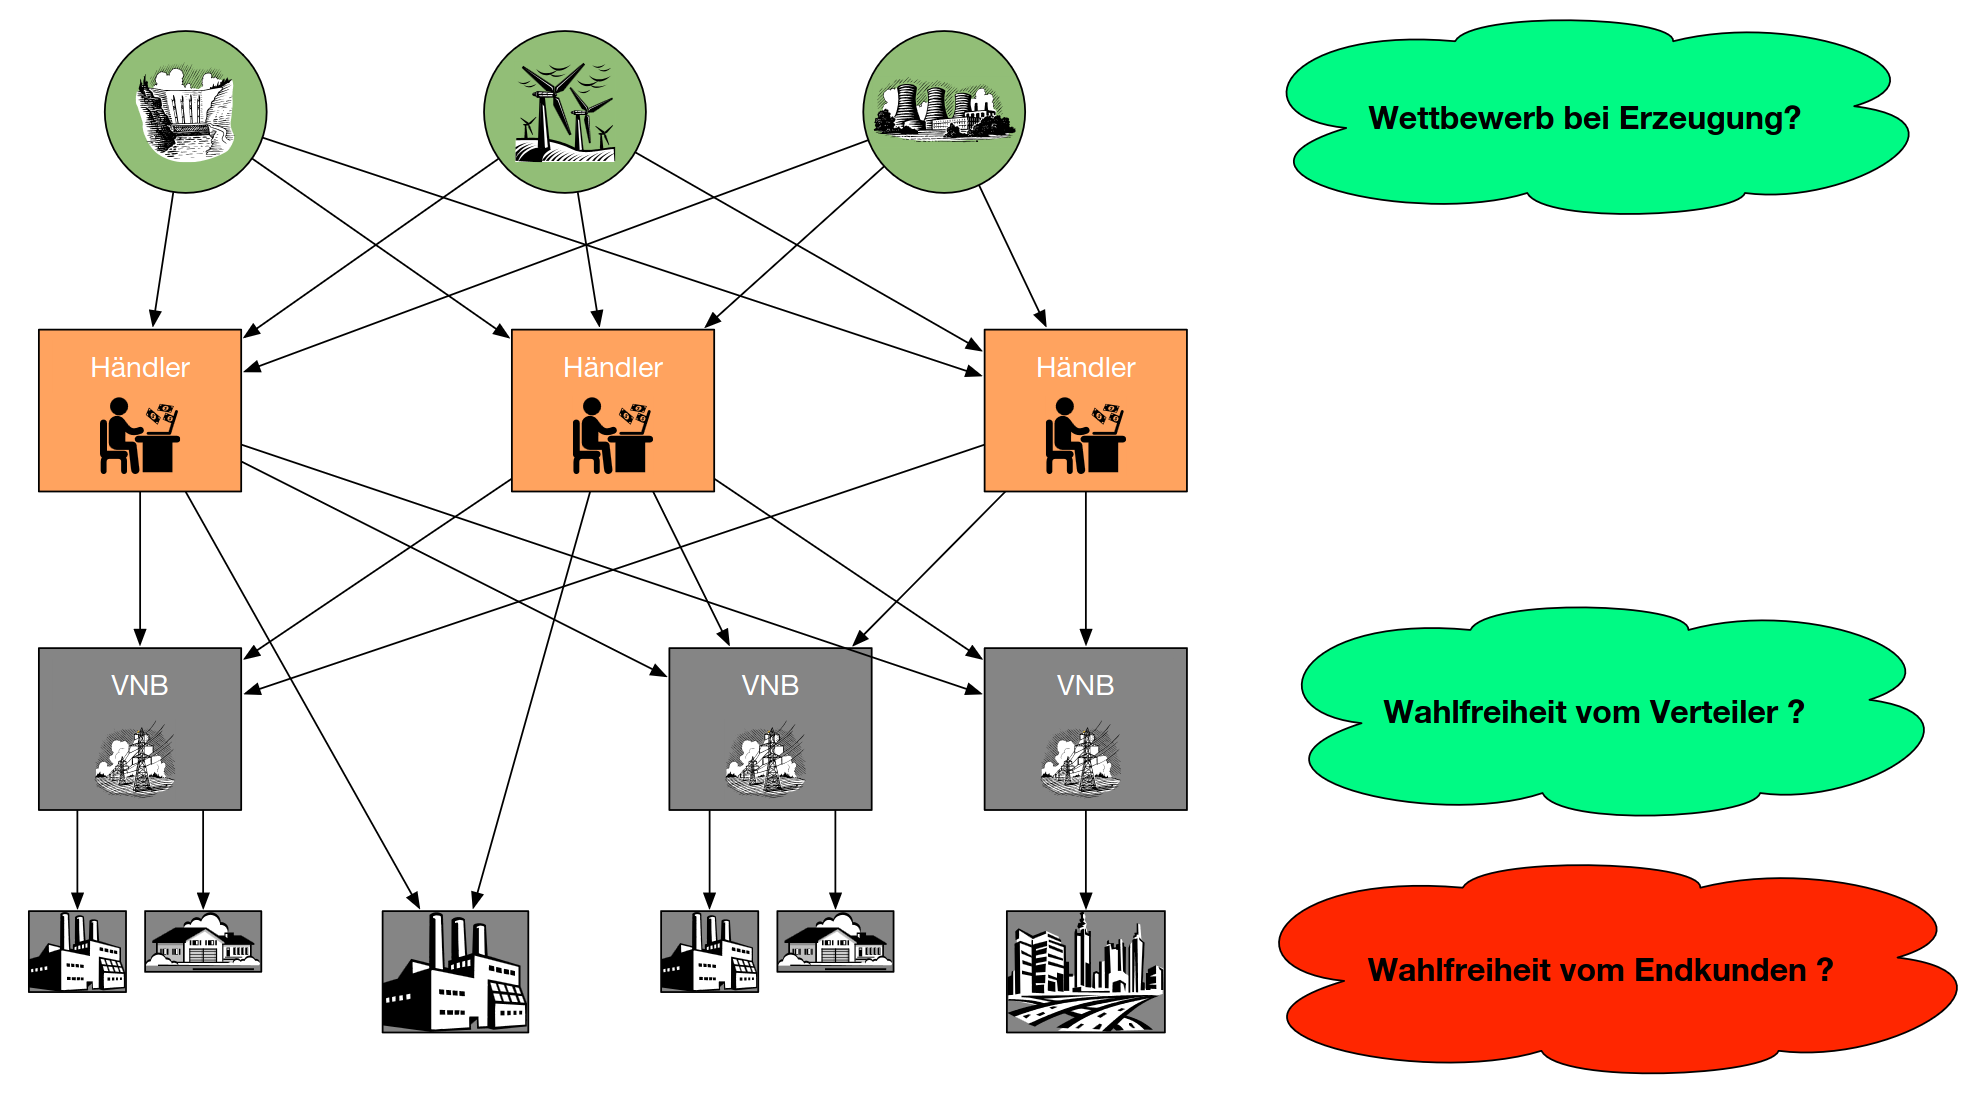
\includegraphics[width=0.95\linewidth]{images/Grosshandel.png}
    \end{minipage}%
    \hfill
    \begin{minipage}[t]{0.49\columnwidth}
        \subsubsection{Vollständiger Wettbewerb}
        \centering \vspace{-0.7\baselineskip}
        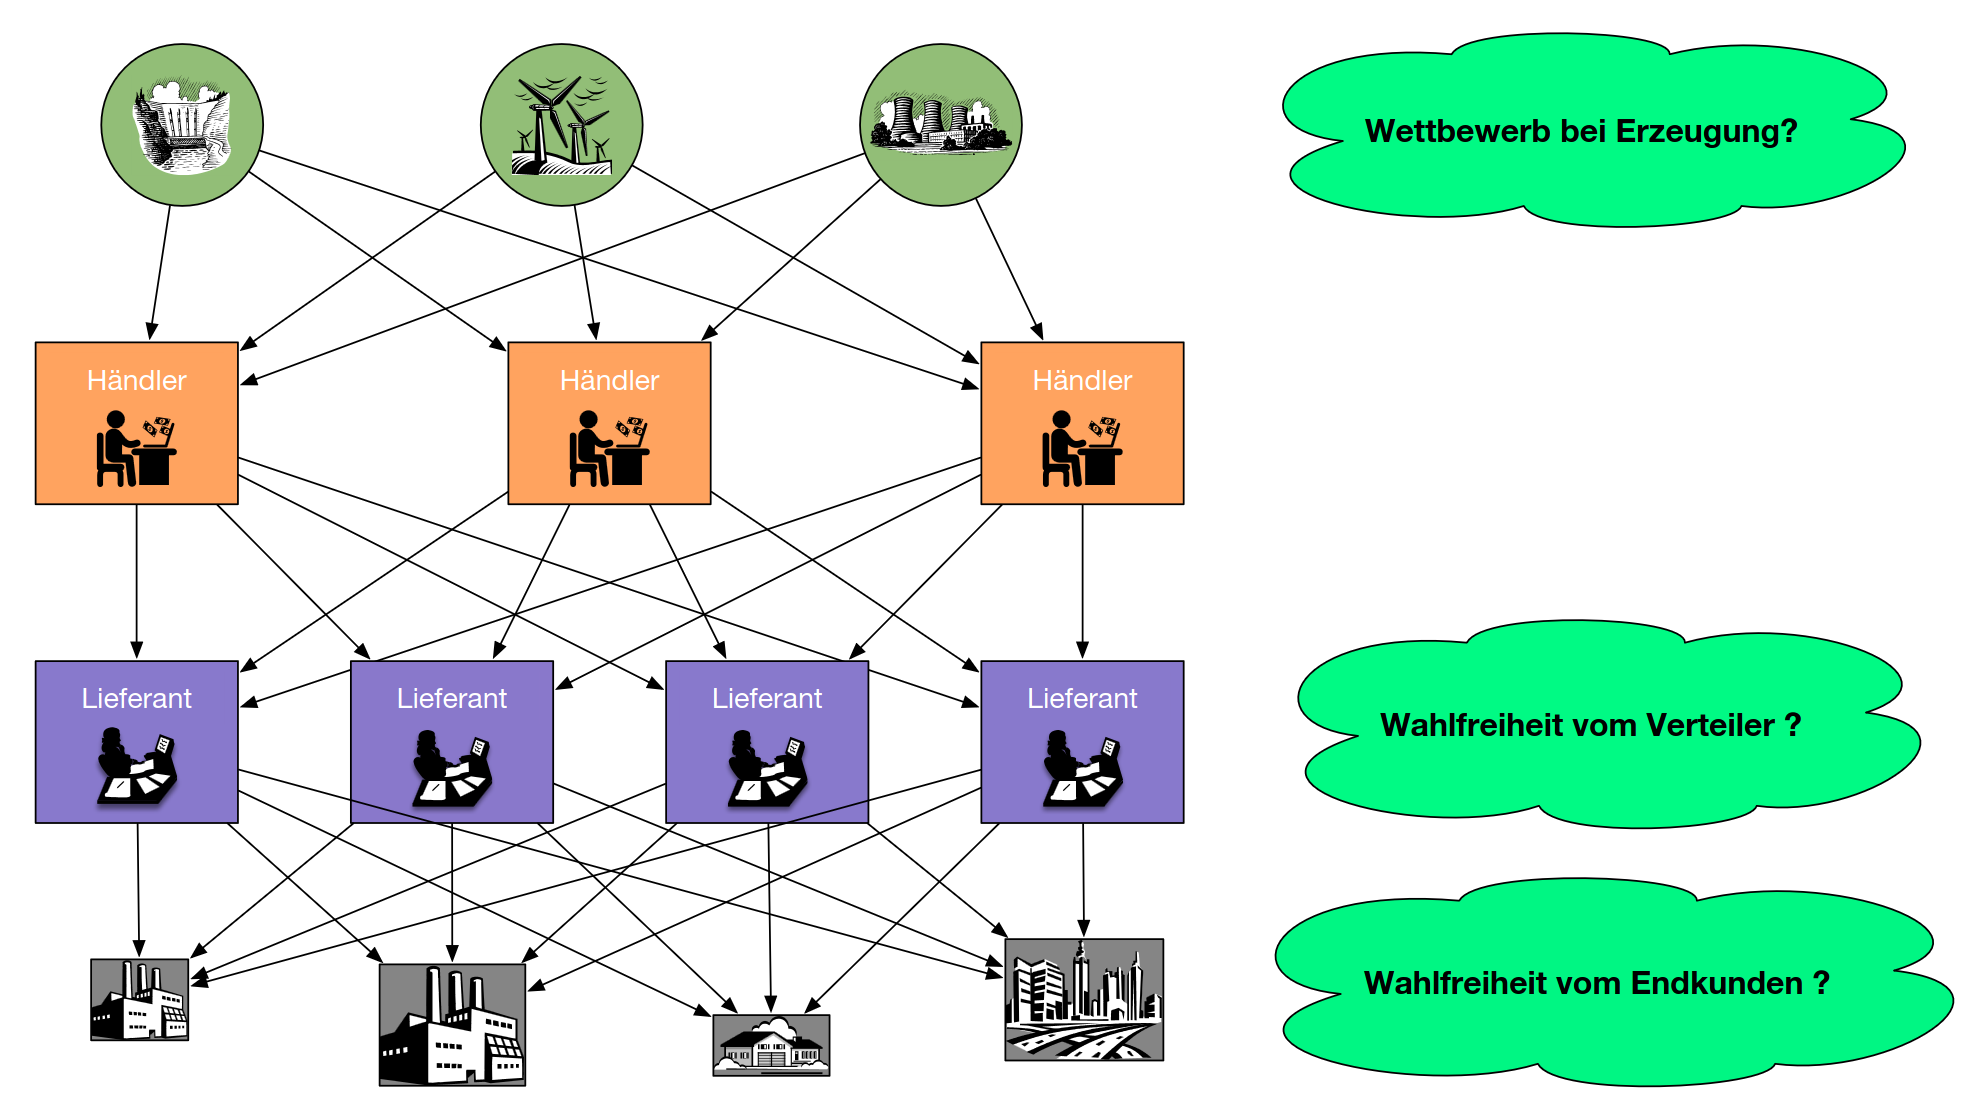
\includegraphics[width=0.95\linewidth]{images/vollst-Wettbewerb.png}
    \end{minipage}

    \subsubsection{Liberalisierung vs. Regulierung}
        \begin{center}
            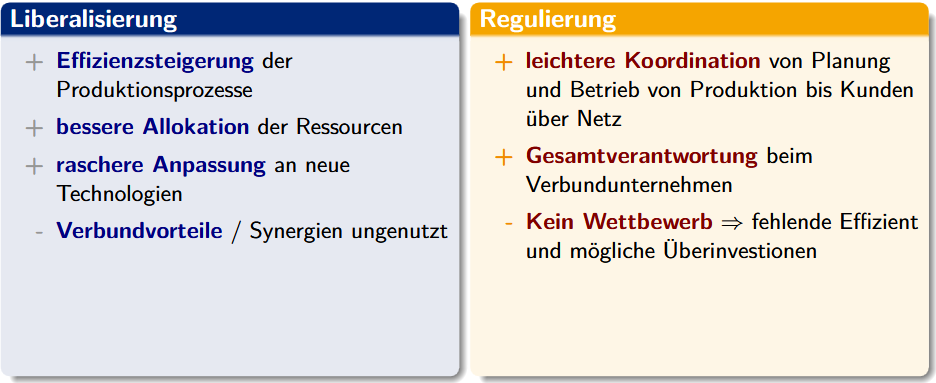
\includegraphics[width=0.8\columnwidth]{images/liberal-regul.png}
        \end{center}

    \subsubsection{Vor der Liberalisierung}
        \begin{minipage}[t]{0.45\columnwidth}
            \centering \vspace{-0.7\baselineskip}
            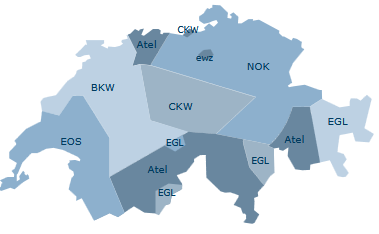
\includegraphics[width=0.95\linewidth]{images/lib-schweiz.png}
        \end{minipage}%
        \hfill
        \begin{minipage}[t]{0.54\columnwidth}
            \begin{itemize}
                \item 7 Verbundunternehmen.
                \item Verbundunternehmen besassen die ganze vertikale Wertschöpfungskette 
                \item[](Erzeugung $\Rightarrow$ Übertragung $\Rightarrow$ Verteilung $\Rightarrow$ Kunde).
                \item Kein Wettbewerb in Versorgungsgebiet
                \item Keine Trennung des Energiegeschäfts
                \item und Transportdienstes
            \end{itemize}
        \end{minipage}

    \subsubsection{Systembetrieb Monopol vs. Wettbewerb}
        \textbf{Monopol:}
        \begin{itemize}
            \item \textbf{Betriebsplanung}          
            \item[] Lang- und kurzfristige Kraftwerkseinsatzplanung und Lastaufteilung             
            \item \textbf{Engpassmanagement}        
            \item[] Bestandteil des Planungsprozesses (Verbundvorteil)                             
            \item \textbf{Spannung \& Frequenz}     
            \item[] Spannungs- und Frequenzregelung als Teil des Planungsprozesses (Verbundvorteil)
            \item \textbf{Nachbetriebliche Prozesse}
            \item[] $-$
        \end{itemize}

        \textbf{Wettbewerbsmarkt:}
        \begin{itemize}
            \item \textbf{Betriebsplanung}          
            \item[] Kraftwerke teilen dem Systembetreiber die Einspeisefahrpläne mit            
            \item \textbf{Engpassmanagement}        
            \item[] Nachträgliche oder iterative Anpassung, falls Marktergebnis zu technisch kritischen Situationen führt                             
            \item \textbf{Spannung \& Frequenz}     
            \item[] Spannungs- und Frequenzregelung mit kontraktierten Regelkraftwerken als Systemdienstleistungen
            \item \textbf{Nachbetriebliche Prozesse}
            \item[] Bereitstellung von Messwerten, Bilanzierung, Abrechnung von Ausgleichsenergie und Regelung
        \end{itemize}

\subsection{Netzsicherheit}
    Ausfall einer Komponente (z.B. Leitung) darf nicht den Ausfall von weiteren Komponenten zur Folge haben $\Rightarrow$
    Keine Ausbreitung von Kaskaden nach Ausfall einer Komponente

\subsubsection{Überwachung der Netzsicherheit}
    \begin{itemize}
        \item Erfassung der Messdaten in den Unterstationen, Übertragung an zentrale Einheit in Echtzeit
        \item Sammlung und Aufbereitung der Messdaten des gesamten Netzes
        \item State Estimation: Estimation des Netzzustands anhand der vorhandenen Messungen (z.B. jede Minute oder nach Ereignis)
        \item Netzsicherheitsrechnung: Beurteilung der (n-1)-Sicherheit (z.B. alle 5 Minuten oder nach Ereignis)
    \end{itemize}

\subsubsection{Beispiel}

\textbf{Maximal:}
\begin{center}
    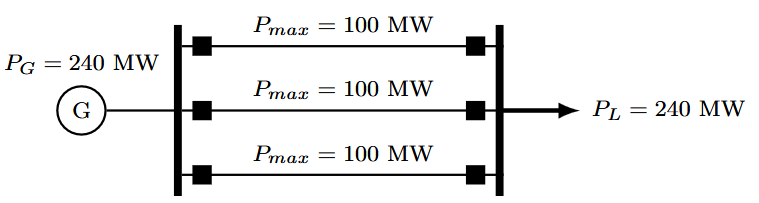
\includegraphics[width=0.7\columnwidth]{images/n-1_maximal.png}
\end{center}

\textbf{Normal:}
\begin{center}
    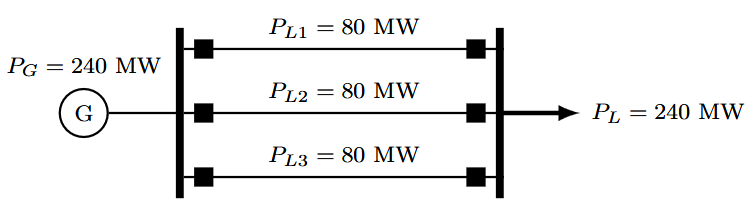
\includegraphics[width=0.7\columnwidth]{images/n-1_normal.png}
\end{center}

\textbf{Fehler:}
\begin{center}
    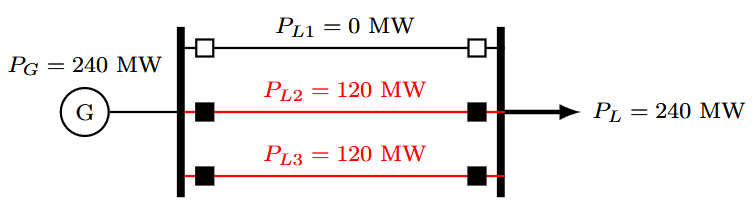
\includegraphics[width=0.7\columnwidth]{images/n-1_fehler.png}
\end{center}

\subsubsection{(N-1)-Sicherheit}
\begin{itemize}
    \item Keine (n-1)-Sicherheit = keine Reserve.
    \item Erst beim Ausfall eines Netzelementes würde ein Problem auftreten.
    \item Solange der Zustand mit n Betriebsmitteln stabil ist, passiert nichts
\end{itemize}

\textbf{Massnahmen:}
\begin{itemize}
    \item Topologische Massnahmen
    \begin{itemize}
        \item Umleitung der Lastflüsse durch Veränderung der Netztopologie
        \item Möglichkeiten
        \item \begin{itemize}
            \item Änderung der Sammelschienenkonfiguration
            \item Stufen von Transformatoren
            \item Zu-/Abschalten von Leitungen und Transformatoren
        \end{itemize}
        \item In der Praxis begrenzter Spielraum
    \end{itemize}
    \item Produktionsverschiebung (Re-Dispatch)
    \begin{itemize}
        \item Gesamtproduktion im Netz anders auf Kraftwerke aufteilen
        \item Gesamtproduktion im Netz erhöhen oder reduzieren
        \item Eingriff in die Produktion = Eingriff in den Markt = grundsätzlich unerwünscht
        \item Volkswirtschaftlicher Schaden, weil das Gleichgewicht des Marktes gestört wird
    \end{itemize}
    \item Lastabwurf
    \begin{itemize}
        \item Gezielte Abschaltung von Lasten
        \item Letztes Mittel zur Rettung des übrigen Netzes
        \item Beispiel: „DSAS” Schweiz - Italien
        \begin{itemize}
            \item DSAS . . . Direct Signal Acquisition System
            \item Bei Überlastung bestimmter Transitleitungen in der Schweiz erfolgt die automatische Abschaltung von Lasten in Italien
            \item Vermeidung von Kaskadenauslösungen
        \end{itemize}
    \end{itemize}
\end{itemize}